\mychapter{Termo de Autorização do Autor}
\label{Cap:anexo}

A principal diferença entre anexo e apêndice é que os apêndices são textos criados pelo próprio autor para complementar sua argumentação, enquanto os anexos são documentos criados por terceiros e usados pelo autor.

Tanto o apêndice quanto o anexo devem estar presentes no sumário dos trabalhos científicos. Os apêndices devem aparecer depois das referências e os anexos depois dos apêndices.

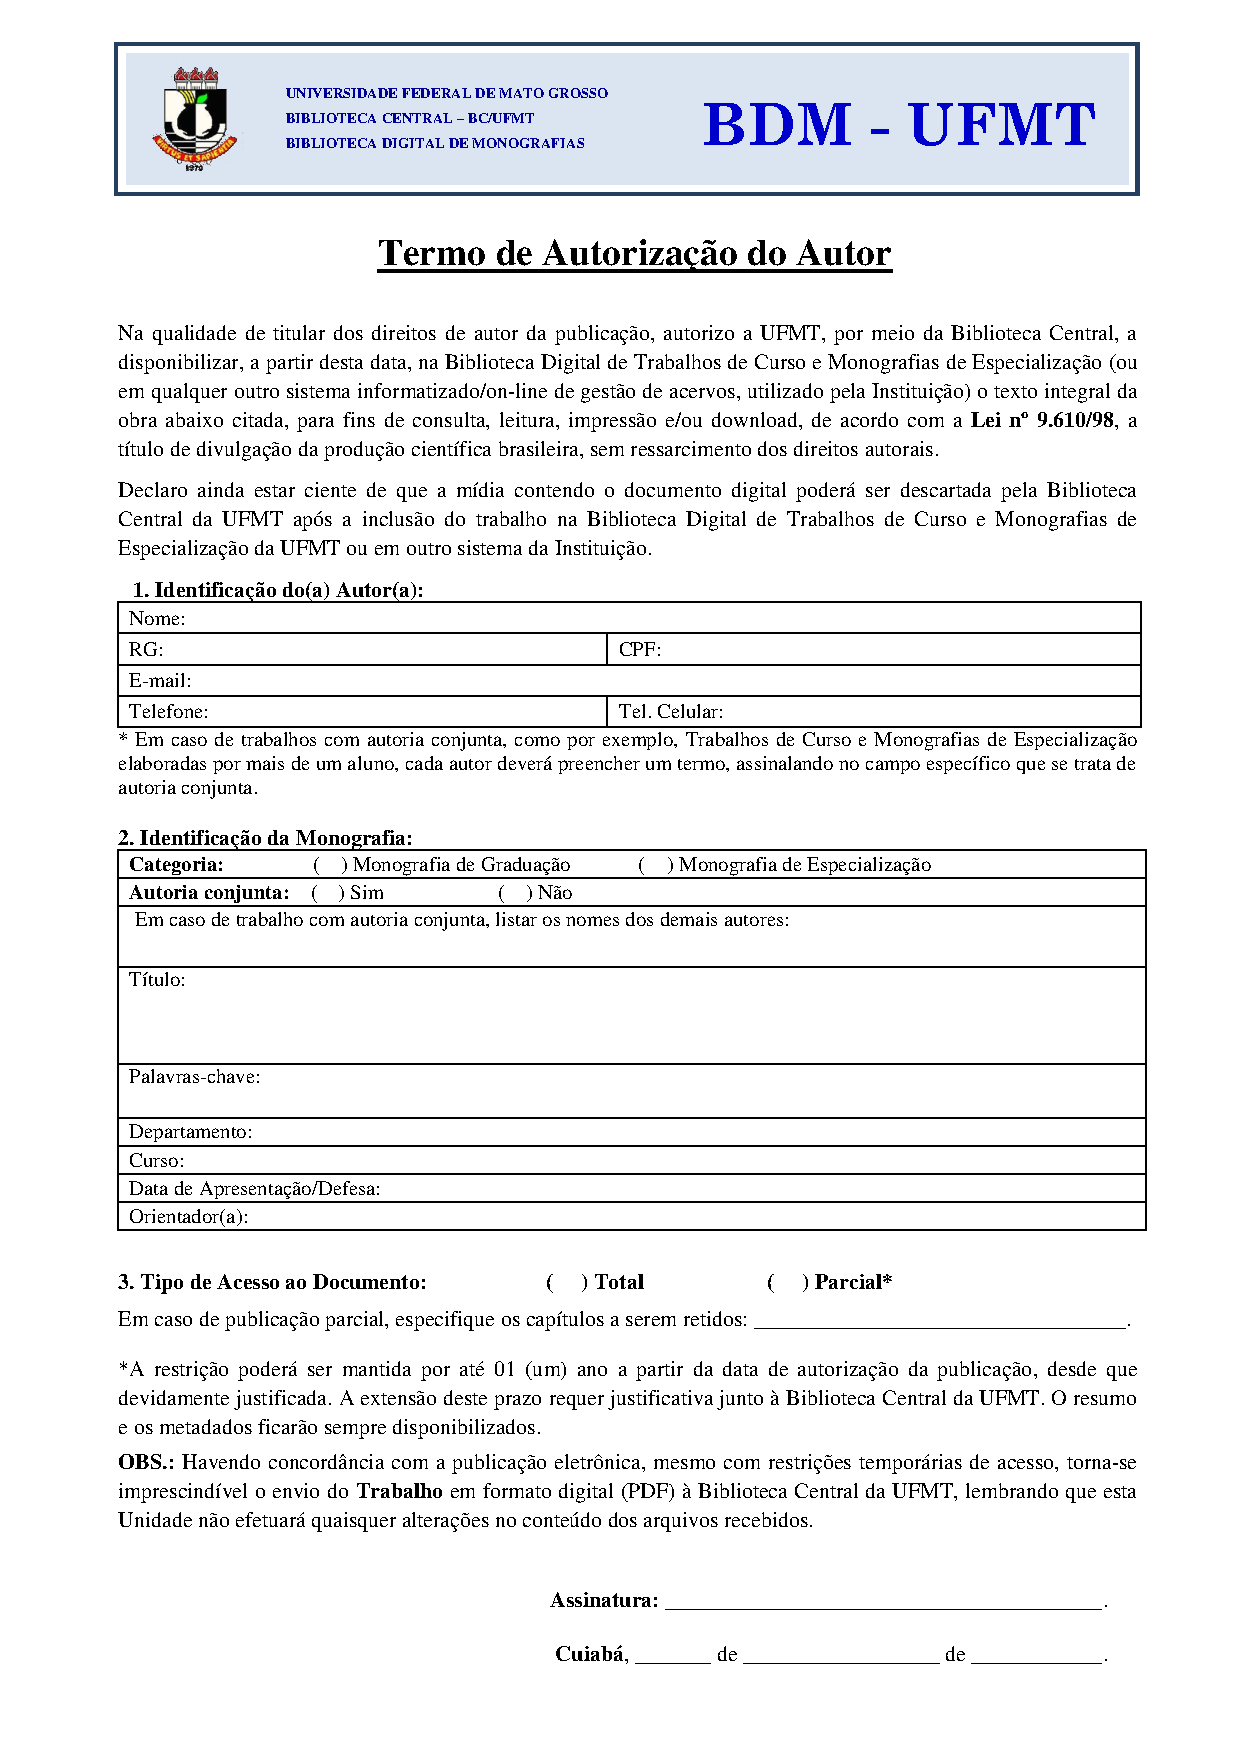
\includepdf[pages=-]{textuais/anexo/termo_de_autorizacao.pdf}
